\documentclass[xetex,mathserif,serif,12pt]{beamer}

\usepackage[orientation=landscape,size=custom,width=16,height=9,scale=.9]{beamerposter}

\usepackage{ifthen}
\usepackage{ifpdf}
\ifpdf
\usepackage{epstopdf}
\fi
\DeclareGraphicsExtensions{.mps,.eps,.png}

\usetheme{iywide}
\setbeamerfont{section in toc}{parent=structure,size=\small}
\setbeamerfont{subsection in toc}{parent=structure,size=\tiny}

\usepackage{hyperref}

\hypersetup{
  colorlinks,%
  citecolor=beamer@solarized@blue,%
  filecolor=beamer@solarized@blue,%
  linkcolor=beamer@solarized@blue,%
  urlcolor=beamer@solarized@blue%
}

\usepackage{fontspec}
\usepackage{xunicode}
\usepackage{xltxtra}
\setmainfont{Ubuntu}
\setmonofont[Scale=0.92]{Inconsolata}

\usepackage[absolute,overlay]{textpos}
\setlength{\TPHorizModule}{1pt}
\setlength{\TPVertModule}{1pt}

\title{A Tour of Go}
\author{Ian Yang}
\institute{Intridea Inc.}

\AtBeginSection[]
{
  \begin{frame}{Outline}
    \tableofcontents[currentsection]
  \end{frame}
}

\usepackage{bibentry}
\nobibliography*
\def\newblock{}

\usepackage{ctable}
\setlength{\heavyrulewidth}{0.1em}
\newcommand{\otoprule}{\midrule[\heavyrulewidth]}

\usepackage{textcomp}
\usepackage{listings}

\begin{document}

\lstdefinelanguage{Go}{
  keywords={type, func, return, defer, go, import, package, var, const, chan, range},
  ndkeywords={len, cap, panic, make},
  sensitive=false,
  comment=[l]{//},
  morecomment=[s]{/*}{*/},
  morestring=[b]',
  morestring=[b]"
}
\lstset{
  language=Go,
  upquote=true,
  columns=fixed,
  numbers=left,
  numberstyle=\tiny\color{beamer@solarized@base01},
  numbersep=9pt,
  tabsize=2,
  extendedchars=true,
  breaklines=true,
  frame=l,
  xleftmargin=4pt,
  framesep=0pt,
  rulesep=10pt,
  framerule=.5pt,
  framexleftmargin=2pt,
  rulecolor=\color{beamer@solarized@base03},
  basicstyle=\footnotesize\ttfamily,
  keywordstyle=\color{beamer@solarized@green},
  stringstyle=\color{beamer@solarized@cyan}\ttfamily,
  identifierstyle=\color{beamer@solarized@blue},
  commentstyle=\color{beamer@solarized@base01},
  emphstyle=\color{beamer@solarized@red}
}

\newcommand{\hltexttt}[1]{\texttt{\color{beamer@solarized@yellow}#1}}

\begin{frame}
  \titlepage
  \begin{textblock}{200}(320,220)
    
\includegraphics{go}
  \end{textblock}
\end{frame}

\section*{Contents}
\begin{frame}{Contents}
  \usebeamerfont{section in toc}
  \tableofcontents
\end{frame}

\section{How to Write Go Code}
\label{sec:how-to-code}

\begin{frame}{How to Write Go Code}

  {\large \href{http://golang.org/doc/code.html}{golang.org/doc/code.html}}

\end{frame}

\begin{frame}[fragile]
  \frametitle{\ttfamily GOPATH}

  \begin{beamer@nomargin}[example text]
    \begin{lstlisting}[language=Bash]
mkdir -p ~/go/src
export GOPATH=~/go
    \end{lstlisting}
  \end{beamer@nomargin}
\end{frame}

\begin{frame}[fragile]
  \frametitle{Directory Structure}

  \begin{beamer@nomargin}[example text]
    \begin{lstlisting}[language=,basicstyle=\small\ttfamily]
go
|- bin
|  `- hello
|- src
|  `- github.com/doitian/studygo
`- pkg
   `- linux_amd64/github.com/doitian/studygo
    \end{lstlisting}
  \end{beamer@nomargin}
\end{frame}

\begin{frame}{Go Package}
  \begin{itemize}[<+->]
  \item All go files in a directory
  \item Do not find files recursively
  \item All files declare the same \hltexttt{package}
  \end{itemize}
\end{frame}

\begin{frame}{Package Search}
  \begin{itemize}[<+->]
  \item Search by import path
  \item Import path is relative directory path
  \item Search paths in \hltexttt{GOPATH} one by one
  \item \hltexttt{pkg} first, then \hltexttt{src}
  \end{itemize}
\end{frame}

\begin{frame}{Executables}
  \begin{itemize}[<+->]
  \item A package that declares \hltexttt{package main}
  \item Installed into \hltexttt{bin}
  \item Run \hltexttt{func main}
  \end{itemize}
\end{frame}

\begin{frame}{Toolkits}
  \begin{itemize}[<+->]
  \item \hltexttt{go build} compile package
  \item \hltexttt{go install} compile and install
  \item \hltexttt{go test} run tests in \hltexttt{*\_test.go}
  \end{itemize}
\end{frame}

\section{A Tour of Go}
\label{sec:tour}

\begin{frame}{A Tour of Go}

  Let's rock with the online tour

  \vskip2ex

  {\LARGE \href{http://tour.golang.org}{tour.golang.org}}

\end{frame}

\subsection{Hello World}
\begin{frame}[fragile]
  \frametitle{Hello World}

  \begin{beamer@nomargin}[example text]
    \begin{lstlisting}[basicstyle=\small\ttfamily]
package main

import "fmt"

func main() {
  fmt.Println("Hello, World")
}
    \end{lstlisting}
  \end{beamer@nomargin}
\end{frame}

\begin{frame}{\ttfamily package}
  \begin{itemize}
  \item Only package \hltexttt{main} is executable
  \item Must be the same in directory
  \item Default name when \hltexttt{import}ed
  \item Convention: same with the last element of the import path
  \end{itemize}
\end{frame}

\begin{frame}[fragile]
  \frametitle{If we do not follow the convention,}

  \begin{beamer@nomargin@title}
    \texttt{\alert{foo}/greeting.go}
  \end{beamer@nomargin@title}

  \begin{beamer@nomargin}[example text]
    \begin{lstlisting}[basicstyle=\small\ttfamily]
package bar // <-- import path is foo
import "fmt"
func Greeting() {
  fmt.Println("Hello, World")
}
    \end{lstlisting}
  \end{beamer@nomargin}
\end{frame}

\begin{frame}[fragile]
  \frametitle{User will be confused.}

  \begin{beamer@nomargin@title}
    \texttt{hello/main.go}
  \end{beamer@nomargin@title}

  \begin{beamer@nomargin}[example text]
    \begin{lstlisting}[basicstyle=\small\ttfamily]
package main
import "foo"
func main() {
  bar.Greeting()
}
    \end{lstlisting}
  \end{beamer@nomargin}
\end{frame}

\begin{frame}[fragile]
  \frametitle{\ttfamily import}

  \begin{beamer@nomargin}[example text]
    \begin{lstlisting}[basicstyle=\small\ttfamily]
import "fmt"
import m "math"

func main() {
  fmt.Println(m.Pi)
}
    \end{lstlisting}
  \end{beamer@nomargin}
\end{frame}

\begin{frame}[fragile]
  \frametitle{in group}

  \begin{beamer@nomargin}[example text]
    \begin{lstlisting}[basicstyle=\small\ttfamily]
import (
  "fmt"
  "math"
)
import (
  fmt "fmt"
  m "math"
)
    \end{lstlisting}
  \end{beamer@nomargin}
\end{frame}

\begin{frame}{Exported names}
  \begin{itemize}
  \item a name is exported if it begins with a capital letter.
  \item global \hltexttt{var}, \hltexttt{const}, \hltexttt{type} and
    \hltexttt{func}
  \end{itemize}
\end{frame}

\begin{frame}{General Declaration Rules}

  \begin{itemize}
  \item type after variable
  \item type is optional if it can be deduced
  \end{itemize}

\end{frame}

\subsection{Functions}

\begin{frame}[fragile]
  \frametitle{\ttfamily func}

  \begin{beamer@nomargin}[example text]
    \begin{lstlisting}
func sum(x int, y int) int {
  return x + y;
}
    \end{lstlisting}
  \end{beamer@nomargin}
\end{frame}

\begin{frame}[fragile]
  \frametitle{\texttt{func} Cont.}

  You can omit the type if two or more consecutive parameters share a type.
  \newline

  \begin{beamer@nomargin}[example text]
    \begin{lstlisting}
func sum(x, y int) int {
  return x + y;
}
    \end{lstlisting}
  \end{beamer@nomargin}
\end{frame}

\begin{frame}[fragile]
  \frametitle{\texttt{func} Multiple results}

  \begin{beamer@nomargin}[example text]
    \begin{lstlisting}
func swap(x, y string) (string, string) {
  return y, x;
}
func main() {
  x, y := swap("hello", "world")
}
    \end{lstlisting}
  \end{beamer@nomargin}
\end{frame}

\begin{frame}[fragile]
  \frametitle{Comma \texttt{ok} pattern}

  \begin{beamer@nomargin}[example text]
    \begin{lstlisting}
func main() {
  m := map[string]string{
    "foo": "bar"
  }

  if name, ok := m["name"]; ok {
    fmt.Println(name)  
  }
}
    \end{lstlisting}
  \end{beamer@nomargin}
\end{frame}

\begin{frame}[fragile]
  \frametitle{Comma \texttt{err} pattern}

  \begin{beamer@nomargin}[example text]
    \begin{lstlisting}
import "os"
import "log"

func main() {
  file, err := os.Open("file.go")
  if err != nil {
    log.Fatal(err)
  }
}
    \end{lstlisting}
  \end{beamer@nomargin}
\end{frame}


\begin{frame}[fragile]
  \frametitle{\texttt{func} Named results}

  \begin{beamer@nomargin}[example text]
    \begin{lstlisting}
func Sqrt(f float64) (result float64, err error) {
  if f < 0 {
    err = ...
  } else {
    result = ...
  }
}
    \end{lstlisting}
  \end{beamer@nomargin}
\end{frame}

\subsection{Variables}

\begin{frame}[fragile]
  \frametitle{Variables}

  The \hltexttt{var} statement declares a list of variables.
  \newline

  \begin{beamer@nomargin}[example text]
    \begin{lstlisting}
var a, b, c int
    \end{lstlisting}
  \end{beamer@nomargin}
\end{frame}

\begin{frame}[fragile]
  \frametitle{Variables Cont.}

  Cross multiple lines
  \newline

  \begin{beamer@nomargin}[example text]
    \begin{lstlisting}
var (
  a int
  b string
)
    \end{lstlisting}
  \end{beamer@nomargin}
\end{frame}

\begin{frame}[fragile]
  \frametitle{Variables initializer}

  \begin{beamer@nomargin}[example text]
    \begin{lstlisting}
var x, y, z = true, "foo", 3.14
    \end{lstlisting}
  \end{beamer@nomargin}
\end{frame}

\begin{frame}[fragile]
  \frametitle{Variables initializer Cont.}

  Cross multiple lines
  \newline

  \begin{beamer@nomargin}[example text]
    \begin{lstlisting}
var (
	a int = 10
	b     = "foo"
)
    \end{lstlisting}
  \end{beamer@nomargin}
\end{frame}

\begin{frame}[fragile]
  \frametitle{Short Assignment}

  \alert{Inside function}, \hltexttt{:=} short assignment statement can
  be used in place of \hltexttt{var} with implicit type.
  \newline

  \begin{beamer@nomargin}[example text]
    \begin{lstlisting}
func main() {
  a, b, c := "foo", true, 3.14
}
    \end{lstlisting}
  \end{beamer@nomargin}
\end{frame}

\begin{frame}
  \frametitle{Variables Scope}

  \begin{itemize}
  \item block scope
  \item parameters and named results are in the scope of function block
  \item \hltexttt{var}, \hltexttt{:=} hide the variable in parent scope
  \end{itemize}
\end{frame}

\begin{frame}

  \frametitle{Primitive Types}

  \begin{itemize}
  \item \hltexttt{bool}
  \item \hltexttt{string}
  \item
    \hltexttt{int}  \hltexttt{int8}  \hltexttt{int16}  \hltexttt{int32}  \hltexttt{int64}\newline
    \hltexttt{uint} \hltexttt{uint8} \hltexttt{uint16} \hltexttt{uint32} \hltexttt{uint64}\newline
    \hltexttt{uintptr}
  \end{itemize}

\end{frame}

\begin{frame}

  \frametitle{Primitive Types Cont.}

  \begin{itemize}
  \item \hltexttt{byte} alias of \hltexttt{uint8}
  \item \hltexttt{rune} Unicode code, alias of \hltexttt{int32}
  \item \hltexttt{float32} \hltexttt{float64}
  \item \hltexttt{complex64} \hltexttt{complex128}
  \end{itemize}
\end{frame}

\begin{frame}[fragile]
  \frametitle{Constants}

  \begin{itemize}
  \item like \hltexttt{var}, but use \hltexttt{const}
  \item character, string, boolean, or numeric values.
  \end{itemize}

  \begin{beamer@nomargin}[example text]
    \begin{lstlisting}
const Pi = 3.14
func main() {
  const World = "world"
}
    \end{lstlisting}
  \end{beamer@nomargin}
\end{frame}

\begin{frame}[fragile]
  \frametitle{First class \texttt{func}}

  \begin{beamer@nomargin}[example text]
    \begin{lstlisting}
add = func(x, y int) int {
  return x + y
}
fmt.Println(add(10, 20)) // => 30
    \end{lstlisting}
  \end{beamer@nomargin}
\end{frame}

\begin{frame}[fragile]
  \frametitle{Closure}

  \begin{beamer@nomargin}[example text]
    \begin{lstlisting}
func adder() func(int) int {
  sum := 0
  return func(int x) int {
    sum += x
    return sum
  }
}
    \end{lstlisting}
  \end{beamer@nomargin}
\end{frame}

\subsection{Control Statements}

\begin{frame}[fragile]
  \frametitle{\ttfamily for}

  \begin{itemize}
  \item no \hltexttt{(} \hltexttt{)}
  \item \hltexttt{\}} \hltexttt{\}} are required
  \end{itemize}

  \begin{beamer@nomargin}[example text]
    \begin{lstlisting}
sum := 0
for i := 1; i <= 10; i++ {
  sum += i
}
    \end{lstlisting}
  \end{beamer@nomargin}
\end{frame}

\begin{frame}[fragile]
  \frametitle{\texttt{for} Pitfalls}

  \begin{itemize}
  \item There is no comma operator
  \item \hltexttt{++} and \hltexttt{--} are statements
  \end{itemize}

  \begin{beamer@nomargin}[example text]
    \begin{lstlisting}
for a,b := 0,0; a<10; a,b = a+1,b+1 {
  ...
}
    \end{lstlisting}
  \end{beamer@nomargin}
\end{frame}

\begin{frame}[fragile]
  \frametitle{\texttt{for} is \texttt{while}}

  \begin{beamer@nomargin}[example text]
    \begin{lstlisting}
sum, i := 0, 1
for i <= 10 {
  sum += i
}
    \end{lstlisting}
  \end{beamer@nomargin}
\end{frame}

\begin{frame}[fragile]
  \frametitle{\texttt{forever}}

  \begin{beamer@nomargin}[example text]
    \begin{lstlisting}
for {
  serve(<-req)
}
    \end{lstlisting}
  \end{beamer@nomargin}
\end{frame}

\begin{frame}[fragile]
  \frametitle{\ttfamily if}

  \vskip-1ex
  \begin{itemize}
  \item no \hltexttt{(} \hltexttt{)}
  \item \hltexttt{\{} \hltexttt{\}} are required
  \end{itemize}

  \begin{beamer@nomargin}[example text]
    \begin{lstlisting}
func abs(x int) int {
  if x < 0 {
    return -x
  }
  return x
}
    \end{lstlisting}
  \end{beamer@nomargin}
\end{frame}

\begin{frame}[fragile]
  \frametitle{\texttt{if} initializer}

  \begin{beamer@nomargin}[example text]
    \begin{lstlisting}
if name, err := m["name"]; ok {
  fmt.Println(name)
}
    \end{lstlisting}
  \end{beamer@nomargin}

  Variable declared in initializer is visible in all branches
\end{frame}

\begin{frame}[fragile]
  \frametitle{Switch}

  \begin{beamer@nomargin}[example text]
    \begin{lstlisting}
switch os := runtime.GOOS; os {
  case "darwin":
    fmt.Println("OS X.")
  case "linux":
    fmt.Println("Linux.")
  default:
    fmt.Printf("%s.", os) // freebsd, ...
  }
}
    \end{lstlisting}
  \end{beamer@nomargin}
\end{frame}

\subsection{Structs}

\begin{frame}[fragile]
  \frametitle{\texttt{struct}}

  \begin{beamer@nomargin}[example text]
    \begin{lstlisting}
type Vertex struct {
    X int
    Y int
}
var origin = Vertex{0, 0}
var xUnit = Vertex{X:1}
var yUnit = Vertex{Y:1}
    \end{lstlisting}
  \end{beamer@nomargin}
\end{frame}

\begin{frame}[fragile]
  \frametitle{\texttt{struct} fields}

  \begin{beamer@nomargin}[example text]
    \begin{lstlisting}
type Vertex struct { X, Y int }
func main() {
  v := Vertex{100, 200}
  v.X = 300
  fmt.Println(v.X, v.Y) // => 300 200
}
    \end{lstlisting}
  \end{beamer@nomargin}
\end{frame}

\begin{frame}[fragile]
  \frametitle{Pointers}

  \begin{beamer@nomargin}[example text]
    \begin{lstlisting}
type Vertex struct { X, Y int }
func main() {
  v := Vertex{100, 200}
  var p *Vertex = &v
  p.X = 300
  fmt.Println(v.X, v.Y) // => 300 200
}
    \end{lstlisting}
  \end{beamer@nomargin}
\end{frame}

\begin{frame}[fragile]
  \frametitle{\texttt{new}}

  \begin{beamer@nomargin}[example text]
    \begin{lstlisting}
var p *T = new(T)
p: = new(T)
    \end{lstlisting}
  \end{beamer@nomargin}
\end{frame}

\subsection{Slices}

\begin{frame}[fragile]
  \frametitle{Slices}

  \begin{beamer@nomargin}[example text]
    \begin{lstlisting}
p := []int{2, 3, 5, 7, 11, 13}

for i := 0; i < len(p); i++ {
  fmt.Printf("p[%d] = %d\n", i, p[i])
}
    \end{lstlisting}
  \end{beamer@nomargin}
\end{frame}

\begin{frame}[fragile]
  \frametitle{Slicing Slices}

  \begin{beamer@nomargin}[example text]
    \begin{lstlisting}
p := []int{2, 3, 5, 7, 11, 13}
p[1:4] // => [3,5,7]
p[1:]  // => [3,5,7,11,13]
p[:4]  // => [2,3,5,7]
    \end{lstlisting}
  \end{beamer@nomargin}
\end{frame}

\begin{frame}[fragile]
  \frametitle{Making slice}

  \begin{beamer@nomargin}[example text]
    \begin{lstlisting}
// make([]T, lenth, capability)
p := make([]int, 0, 10)
cap(p) // => 10
len(p) // => 0
    \end{lstlisting}
  \end{beamer@nomargin}
\end{frame}

\begin{frame}[fragile]
  \frametitle{Slicing beyond \texttt{len}}

  \begin{beamer@nomargin}[example text]
    \begin{lstlisting}
p := make([]int, 5, 10)
p = p[3,8] // len(p)=5,cap(p)=7
    \end{lstlisting}
  \end{beamer@nomargin}
\end{frame}

\begin{frame}[fragile]
  \begin{beamer@nomargin}[example text]
    \begin{lstlisting}
p := make([]int, 5, 10)
    \end{lstlisting}
  \end{beamer@nomargin}
  \vskip-.1ex

   \begin{beamer@nomargin}
   \begin{figure}
     \centering
     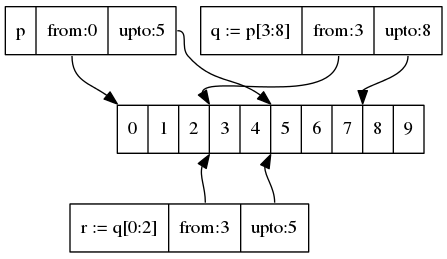
\includegraphics[height=7.35cm]{slice}
     \label{fig:slice}
   \end{figure}
   \end{beamer@nomargin}
\end{frame}

\begin{frame}[fragile]
  \frametitle{\texttt{range}}

  \begin{beamer@nomargin}[example text]
    \begin{lstlisting}
pow := make([]int, 10)
for i := range pow {
  pow[i] = 1 << uint(i)
}
for _, value := range pow {
  fmt.Printf("%d\n", value)
}
for i, value := range pow {
  fmt.Printf("pow[%d]=%d\n", i, value)
}
    \end{lstlisting}
  \end{beamer@nomargin}
\end{frame}

\subsection{Maps}

\begin{frame}[fragile]
  \frametitle{\texttt{map}}

  \begin{beamer@nomargin}[example text]
    \begin{lstlisting}
type Vertex struct {
  Lat, Long float64
}

var m = map[string]Vertex{
  "Bell Labs": Vertex{40.68433, -74.39967},
  "Google": Vertex{37.42202, -122.08408},
}
    \end{lstlisting}
  \end{beamer@nomargin}
\end{frame}

\begin{frame}[fragile]
  \frametitle{\texttt{map} Cont.}

  \begin{beamer@nomargin}[example text]
    \begin{lstlisting}
type Vertex struct {
  Lat, Long float64
}

var m = map[string]Vertex{
  "Bell Labs": 40.68433, -74.39967,
  "Google": 37.42202, -122.08408,
}
    \end{lstlisting}
  \end{beamer@nomargin}
\end{frame}

\begin{frame}[fragile]
  \frametitle{\texttt{map} functions}

  \begin{beamer@nomargin}[example text]
    \begin{lstlisting}
m[key] = value
elem = m[key]
delete(m, key)
elem, ok = m[key]
    \end{lstlisting}
  \end{beamer@nomargin}
\end{frame}

\subsection{Methods}

\begin{frame}[fragile]
  \frametitle{Methods}

  \begin{beamer@nomargin}[example text]
    \begin{lstlisting}
type Vertex struct{ X, Y float64 }
func (v *Vertex) double() {
  v.X, v.Y = v.X*2, v.Y*2
}

func main() {
  v := &Vertex{1, 2}
  v.double() // => &Vertex{2,4}
}
    \end{lstlisting}
  \end{beamer@nomargin}
\end{frame}

\begin{frame}[fragile]
  \frametitle{Revisit Pointer}

  \begin{beamer@nomargin}[example text]
    \begin{lstlisting}
type Vertex struct{ X, Y float64 }
func (v Vertex) double() {
  v.X, v.Y = v.X*2, v.Y*2
}

func main() {
  v := &Vertex{1, 2}
  v.double() // => &Vertex{1,2}
}
    \end{lstlisting}
  \end{beamer@nomargin}
\end{frame}

\begin{frame}
  \frametitle{Revisit Pointer Cont.}

  \begin{itemize}
  \item You can pass pointer when value is required
  \item You can pass value when pointer is required only as method receiver (maybe a bug)
  \end{itemize}
\end{frame}

\begin{frame}
  \frametitle{Methods Cont.}

  \begin{itemize}
  \item In fact, you can define a method on any type you define in your package, not just \hltexttt{struct}s.
  \item You cannot define a method on a type from another package, or on a basic type.
  \end{itemize}
\end{frame}

\begin{frame}[fragile]
  \frametitle{Methods Cont.}

  \begin{beamer@nomargin}[example text]
    \begin{lstlisting}
type SqrtError float64

func (err SqrtError) Error() string {
  return fmt.Sprintf("Sqrt: %v is nagative", float64(err))
}
    \end{lstlisting}
  \end{beamer@nomargin}
\end{frame}

\subsection{Interfaces}

\begin{frame}
  \frametitle{Interfaces}

  \begin{itemize}
  \item An interface type is defined by a set of methods.
  \item A value of interface type can hold any value that implements those methods.
  \end{itemize}
\end{frame}

\begin{frame}[fragile]
  \frametitle{Interfaces}

  \begin{beamer@nomargin}[example text]
    \begin{lstlisting}
type error interface {
  Error() string
}
    \end{lstlisting}
  \end{beamer@nomargin}
\end{frame}

\begin{frame}[fragile]
  \frametitle{Interfaces}

  \begin{beamer@nomargin}[example text]
    \begin{lstlisting}
type SqrtError float64
func (err *SqrtError) Error() string {
	return fmt.Sprintf("Sqrt: %v is nagative", float64(*err))
}
var err = SqrtError(3)
var x error = 1 // => type error
var y error = err // => type error
var z error = &err // => OK
    \end{lstlisting}
  \end{beamer@nomargin}
\end{frame}

\begin{frame}
  \frametitle{Interfaces and Pointer}

  \begin{itemize}
  \item Methods defined on value is considered defined on pointer as well
  \item Methods defined on pointer is not defined on value
  \end{itemize}
\end{frame}

\begin{frame}[fragile]
  \frametitle{Interfaces and Pointer}

  \begin{beamer@nomargin}[example text]
    \begin{lstlisting}
type SqrtError float64
func (err SqrtError) Error() string {
	return fmt.Sprintf("Sqrt: %v is nagative", float64(err))
}
var err = SqrtError(3)
var x error = 1 // => type error
var y error = err // => OK
var z error = &err // => OK
    \end{lstlisting}
  \end{beamer@nomargin}
\end{frame}


\begin{frame}[fragile]
  \frametitle{Interfaces Union}

  \begin{beamer@nomargin}[example text]
    \begin{lstlisting}
type ReadWriter interface {
    Reader
    Writer
}
    \end{lstlisting}
  \end{beamer@nomargin}
\end{frame}

\begin{frame}[fragile]
  \frametitle{Embedding}

  \begin{beamer@nomargin}[example text]
    \begin{lstlisting}
type Job struct {
  Command string
  *log.Logger
}
    \end{lstlisting}
  \end{beamer@nomargin}

  \hltexttt{Job} has all methods defined on \hltexttt{log.Logger}.
\end{frame}

\begin{frame}[fragile]
  \frametitle{Embedding}
  Last part of the type name is defined as implicit field name

  \begin{beamer@nomargin}[example text]
    \begin{lstlisting}
func main() {
  job := Job{Logger: log.New(os.Stderr, "Job: ", log.Ldate)}

  fmt.Println(job)
}
    \end{lstlisting}
  \end{beamer@nomargin}
\end{frame}

\subsection{Concurrency}

\begin{frame}[fragile]
  \frametitle{Goroutines}

  A goroutine is a lightweight thread 
  \newline

  \begin{beamer@nomargin}[example text]
    \begin{lstlisting}
go f(x, y, z)
    \end{lstlisting}
  \end{beamer@nomargin}

\end{frame}

\begin{frame}[fragile]
  \frametitle{Channels}

  Channels are a typed conduit through which you can send and receive values
  with the channel operator, \hltexttt{<-}.\newline

  \begin{beamer@nomargin}[example text]
    \begin{lstlisting}
ch <- v   // send v to channel
v := <-ch // receive from ch, and assign to v
    \end{lstlisting}
  \end{beamer@nomargin}
\end{frame}

\begin{frame}[fragile]
  \frametitle{Makeing Channels}
  \begin{beamer@nomargin}[example text]
    \begin{lstlisting}
ch := make(chan int)
queue = make(chan *Request)
    \end{lstlisting}
  \end{beamer@nomargin}
\end{frame}

\begin{frame}
  \frametitle{Channels Blocking}

  \begin{itemize}
  \item sender is blocked until data is read by receiver
  \item receiver is blocked until data is placed by sender
  \end{itemize}
\end{frame}

\begin{frame}[fragile]
  \frametitle{Buffered Channels}
  \begin{beamer@nomargin}[example text]
    \begin{lstlisting}
ch := make(chan int, 10)
queue = make(chan *Request, 100)
    \end{lstlisting}
  \end{beamer@nomargin}
\end{frame}

\begin{frame}
  \frametitle{Buffered Channels Blocking}

  \begin{itemize}
  \item sender is blocked when buffer is full
  \item receiver is blocked when buffer is empty
  \end{itemize}
\end{frame}

\begin{frame}[fragile]
  \begin{beamer@nomargin}[example text]
    \begin{lstlisting}
func worker(a []int, ch chan int) {
  result := sum(a)
  ch <- result
}

func main() {
  ch := make(chan int)
  go worker([]int{1, 2, 3, 4, 5, 6, 7, 8, 9, 10}, ch)

  fmt.Println(<-ch) // => 3
}
    \end{lstlisting}
  \end{beamer@nomargin}
\end{frame}

\begin{frame}[fragile]
  \frametitle{\ttfamily select}

  \begin{beamer@nomargin}[example text]
    \begin{lstlisting}
select {
case c <- x:
  x, y = y, x+y
case <-quit:
  fmt.Println("quit")
  return
}
    \end{lstlisting}
  \end{beamer@nomargin}
\end{frame}

\begin{frame}[fragile]
  \frametitle{non-blocking {\ttfamily select}}

  \begin{beamer@nomargin}[example text]
    \begin{lstlisting}
select {
case c <- x:
  x, y = y, x+y
case <-quit:
  fmt.Println("quit")
  return
default:
  time.Sleep(5e7)
}
    \end{lstlisting}
  \end{beamer@nomargin}
\end{frame}

\section{Continue Reading}

\begin{frame}{Continue Reading}
  \begin{itemize}
  \item \href{http://golang.org/doc/effective_go.html}{Effective Go}
  \item \href{http://golang.org/doc/articles/defer_panic_recover.html}{Defer,
      Panic, and Recover} (similar to exception)
  \item
    \href{http://golang.org/doc/articles/concurrency_patterns.html}{Concurrency
      Patterns}
  \item \href{http://golang.org/pkg/}{Packages Reference}
\end{itemize}
\end{frame}

\end{document}
